%!TEX root = thesis.tex

\chapter{Introduction}

Operating a robot and developing high level control code for it is a cumbersome task. Very often various groups of developers are working simultaneously on different parts of the software. But in most cases there is only one device that can be used for testing and so only one can run his/her code at a time. The others have to wait until they get access to the robot. Moreover, tests on real robots always come with a high level of risk. Incorrect algorithms can lead very fast to damages on robot components or their environment and entail costly repairs. In the worst case even people can get hurt by uncontrolled robot motions.

The solution to those problems is the usage of a simulator that mimics the robot components and their behavior as accurate as possible. It has to provide the same control interface so that each part of the software can get tested on the simulator before it gets utilized on the real robot. Those considerations motivated the first part of this thesis -- the realistic replication of the IIS-Lab robot setup on a suitable simulation platform. This involves the creation of an exact model of the robot setup, containing the various robot components and their environment. The necessary steps are explained in Chapter~\ref{chap:simulation}.

The second part of the thesis is about motion planning. Moving the robot hand cannot follow any arbitrary trajectory towards a target pose. During that motion it might collide with itself or any other obstacle within it's environment. That means those trajectories have to be planned carefully to avoid accidental collisions and to generate smooth and well controlled robot motions. This also involves to create and maintain an internal representation of the robot and it's environment, a step that is common to the simulation part of the thesis. Chapter 3 shows the configuration and integration of the motion planning framework MoveIt into the IIS-Lab robot setup along with some usage examples.

Chapter 4 focuses on MoveIt's grasping functionality. It shows, how a reference `Pick and Place' task can be planned with the planning tools  and executed on the simulator and the real robot as well.

In Chapter 5, some test results will be presented, analyzing the quality of the various planning algorithms and approaches.

\section{IIS-Lab Robot Setup}
\begin{figure}[ht]
	\centering
  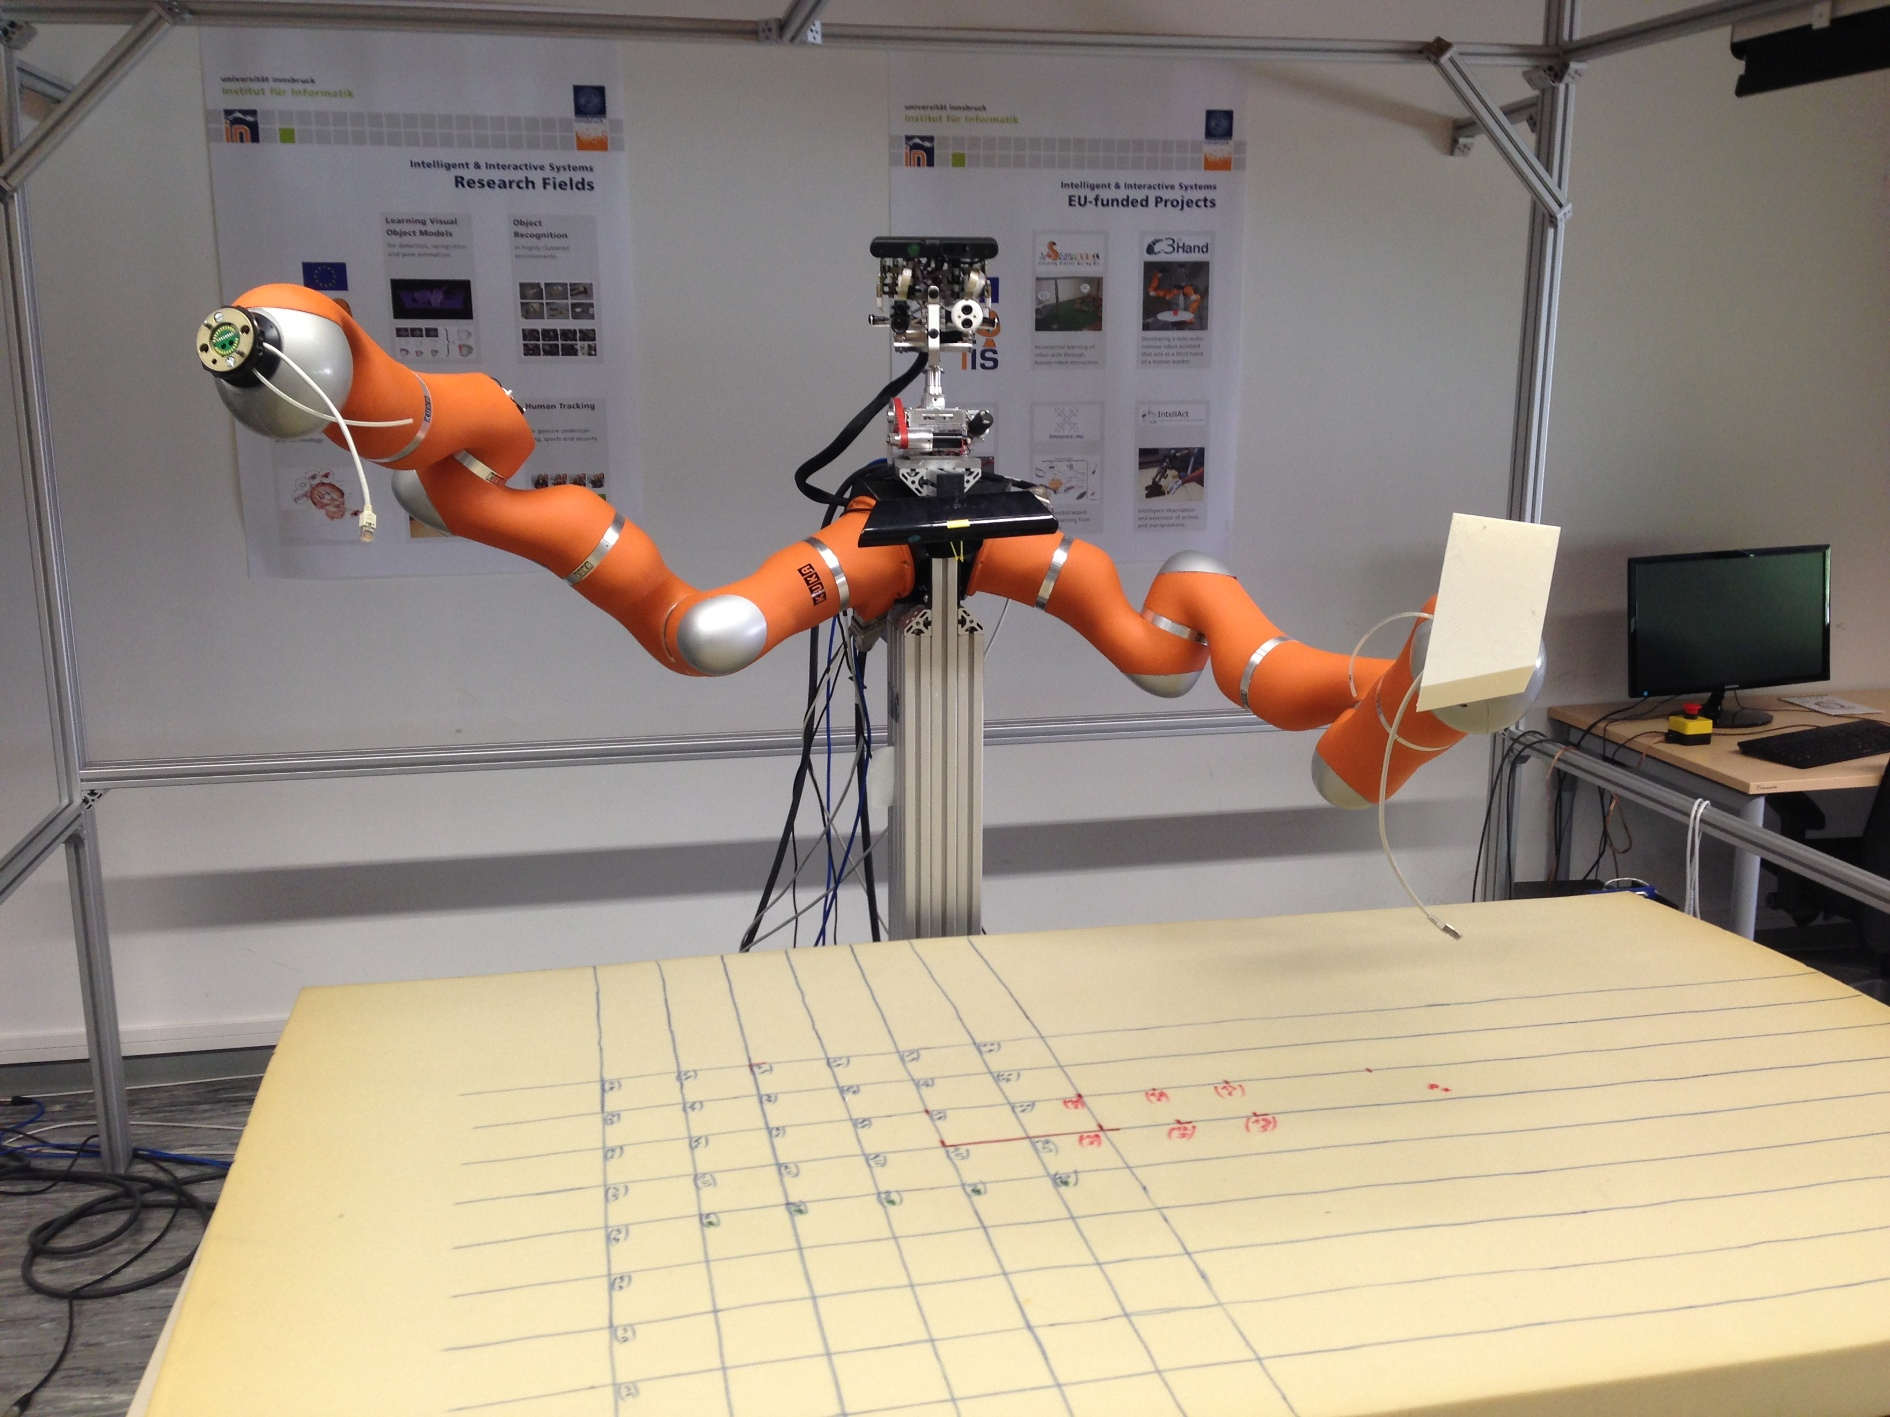
\includegraphics[width=0.75\textwidth]{images/robot_setup.jpg}
	\caption{Current setup in the IIS-Lab TODO: provide more recent image}
	\label{fig:fig1}
\end{figure}

The robot setting, that was considered in this thesis can be seen in Figure \ref{fig:fig1}
The main part of the robot setup in the IIS-Lab consists of an aluminium torso with two mounted KUKA light weight robot arms. Those arms have 7 degrees of freedom (DOF) each one can carry up to 7kg of payload. Additionally a Schunk SDH gripper can be mounted on each arm.

\begin{itemize}
	\item \textbf{KUKA LWR 4+ arm}\\
		Description of the arm(7 DOF, max. 7kg payload, 16kg weight, very flexible,...
	\item \textbf{Schunk SDH gripper}\\
		Description of the gripper(3-finger-gripper, different grasp types, as powerful as human hand, very sensitive)
	\item \textbf{Kinect camera}\\
		Description of Kinect(RGB camera, Depth sensor, 3d data under any light conditions)
\end{itemize}


\section{The Robot Operating System(ROS)}

The implementation of the project requirements is based on ROS. Therefore a brief introduction about the basic concepts\footnote{http://wiki.ros.org/ROS/Concepts} shall be given here. The explained terminology will be used throughout this thesis. As stated in \cite{quigley2009}, ROS is not an operating system in the classical sense. It runs on top of a host operating system (usually linux) and can be seen as an additional communication layer, providing various mechanisms for inter process communication. A ROS system consists of a number of \emph{nodes}. Each node is an independent computation unit that runs in it's own process, adding some clearly defined functionality to the overall system. For example one node can be responsible for planning, another one for perception and a third one for controlling the hardware. Nodes communicate to each other by passing \emph{messages}, using the ROS communication infrastructure. Messages are strictly typed data structures, defined in a special message composition format\footnote{http://wiki.ros.org/msg}. They can be composed of primitive types like float, integer or string, but also of other message types. Therefore it is possible to create arbitrary complex messages for each use case. Messages are published to \emph{topics}. A topic is a strongly typed message bus, addressed by it's \emph{topic name}. Arbitrary nodes can connect to a topic in parallel, as long as they use the correct message type. Each node can publish and subscribe to a number of topics. It is also possible that various nodes publish to the same topic. 

Topic names are strings, used to identify topics. They can be organized into \emph{namespaces} to build a tree hierarchy comparable to the directory structure in a file system. This is very important, as for example the simulator should use similar topic names as the real robot. The namespace concept allows both instances to use identical names but each one in it's own namespace. The following samples represent valid topic names:
\begin{itemize}
\item \texttt{/} (this is the root namespace)
\item \texttt{/topic}
\item \texttt{/component/topic}
\item \texttt{/namespace/component/topic}
\end{itemize}

The communication via ROS topics is asynchronous - involved nodes may even not be aware of each others existence. Synchronous message exchange between nodes happens via ROS \emph{services}. In contrast to topics, a service with a given name can only be offered by one single node. Services are addressed, using the same naming strategy as topics. The service message is composed of a request and a response part. A client node that sends a service request will block, until the advertising node has handled the request and delivers a response. The concept of ROS topics and services is shown in Figure \ref{fig:ros_concept}
\begin{figure}[h]
	\centering
  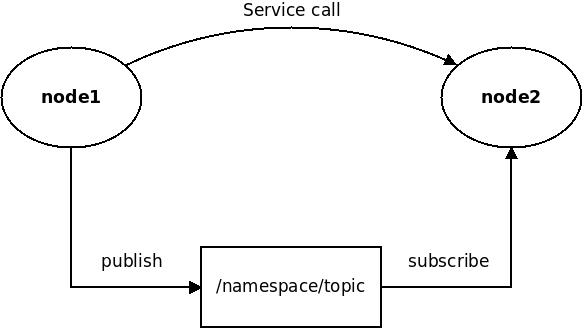
\includegraphics[width=0.5\textwidth]{images/ros_concept.jpg}
	\caption{ROS nodes, topics and services}
	\label{fig:ros_concept}
\end{figure}

The nodes of a ROS system can be distributed over various different machines. One of them has to be the dedicated \emph{ROS master}. The master is responsible to handle topic and service registrations and holds information about the involved ROS nodes. Other machines connect to the master via network. The ROS master also provides a centralized \emph{parameter server}. This is a shared dictionary that can be used to store and retrieve configuration data and other shared parameters. Nodes can access the parameter server at runtime and read or modify it's content. \\

A system usually consists of a large number of nodes that have to be configured and started. This can be done, using so called \emph{launch files}. Those are simple textfiles, holding startup information and configuration details for one or more nodes in an XML like syntax. Using the \emph{roslaunch} command line tool, a whole system of nodes can be configured and launched at once. \\

ROS is a modular software system organized into \emph{packages}. Each package adds clearly defined functionality and can be reused in other systems. Packages can be installed on demand and they may also depend on the functionality of other packages. A package might contain one or more ROS nodes or even only configuration data. Additional packages can be downloaded and installed, using a package manager tool.
Custom functionality is added to a ROS system by creating a new package and developing the required piece of software.

\section{Project Targets}
Both objectives

	\begin{itemize}
	
		\item \textbf{Simulation}\\
			Realistic replication of the robot setup on a suitable simulation platform
			Generation of realistic sensor data
			Visualization of collisions
			Implementation of a ROS interface, corresponding to that one of the real robot
		\item \textbf{Motion Planning}\\
			Configuration and integration of a motion planning framework
			Implementation of a benchmark pick and place task, executable on simulator and
			real robot
			Provide an easy to use interface to the planner
			Analyse the quality of the various planning algorithms
			
	\end{itemize}